\chapter{Graphen}

Ein Graph ist eine mathematische Struktur zur Darstellung von Beziehungen zwischen Objekten.
Die Idee, Objekte durch Verknüpfungen zu verbinden, bildet die Grundlage für zahlreiche Anwendungen, unter anderem die Routenplanung.
Graphen und insbesondere kürzeste Pfade spielen darüber hinaus eine wichtige Rolle; in einem Wissensgraphen kann ein Pfad etwa die Gültigkeit einer Aussage repräsentieren.
\autoref{graphs:fig:beispielgraph} zeigt einen Graphen, der im Folgenden für Beispiele verwendet wird.

\begin{figure}[ht]
  \centering
  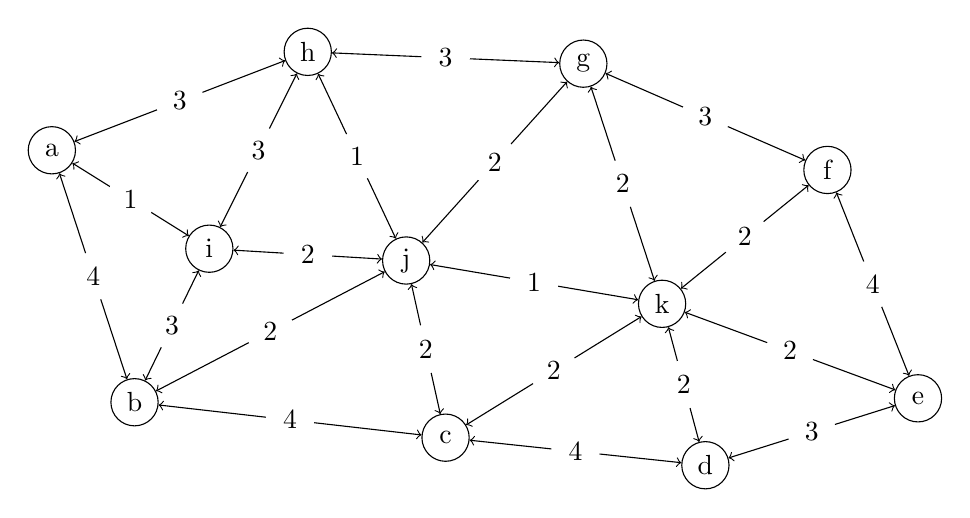
\begin{tikzpicture}
    % Nodes
    \node[circle, draw, minimum size=0.6cm, inner sep=0pt] at (0.5* 0.0, 0.5* 8.5)  (a)    {a};
    \node[circle, draw, minimum size=0.6cm, inner sep=0pt] at (0.5* 2.1, 0.5* 2.1)  (b)    {b};
    \node[circle, draw, minimum size=0.6cm, inner sep=0pt] at (0.5* 10.0, 0.5* 1.2)  (c)    {c};
    \node[circle, draw, minimum size=0.6cm, inner sep=0pt] at (0.5* 16.6, 0.5* 0.5)  (d)    {d};
    \node[circle, draw, minimum size=0.6cm, inner sep=0pt] at (0.5* 22.0, 0.5* 2.2)  (e)    {e};
    \node[circle, draw, minimum size=0.6cm, inner sep=0pt] at (0.5* 19.7, 0.5* 8.0)  (f)    {f};
    \node[circle, draw, minimum size=0.6cm, inner sep=0pt] at (0.5* 13.5, 0.5* 10.7)  (g)    {g};
    \node[circle, draw, minimum size=0.6cm, inner sep=0pt] at (0.5* 6.5, 0.5* 11.0)  (h)    {h};
    \node[circle, draw, minimum size=0.6cm, inner sep=0pt] at (0.5* 4.0, 0.5* 6.0)  (i)    {i};
    \node[circle, draw, minimum size=0.6cm, inner sep=0pt] at (0.5* 9.0, 0.5* 5.7)  (j)    {j};
    \node[circle, draw, minimum size=0.6cm, inner sep=0pt] at (0.5* 15.5, 0.5* 4.6)  (k)    {k};

    \draw[<->]  (a) edge node[circle, fill=white] {4} (b);
    \draw[<->]  (a) edge node[circle, fill=white] {3} (h);
    \draw[<->]  (a) edge node[circle, fill=white] {1} (i);

    \draw[<->]  (b) edge node[circle, fill=white] {4} (c);
    \draw[<->]  (b) edge node[circle, fill=white] {3} (i);
    \draw[<->]  (b) edge node[circle, fill=white] {2} (j);

    \draw[<->]  (c) edge node[circle, fill=white] {4} (d);
    \draw[<->]  (c) edge node[circle, fill=white] {2} (j);
    \draw[<->]  (c) edge node[circle, fill=white] {2} (k);

    \draw[<->]  (d) edge node[circle, fill=white] {3} (e);
    \draw[<->]  (d) edge node[circle, fill=white] {2} (k);

    \draw[<->]  (e) edge node[circle, fill=white] {4} (f);
    \draw[<->]  (e) edge node[circle, fill=white] {2} (k);

    \draw[<->]  (f) edge node[circle, fill=white] {3} (g);
    \draw[<->]  (f) edge node[circle, fill=white] {2} (k);

    \draw[<->]  (g) edge node[circle, fill=white] {3} (h);
    \draw[<->]  (g) edge node[circle, fill=white] {2} (j);
    \draw[<->]  (g) edge node[circle, fill=white] {2} (k);

    \draw[<->]  (h) edge node[circle, fill=white] {3} (i);
    \draw[<->]  (h) edge node[circle, fill=white] {1} (j);

    \draw[<->]  (i) edge node[circle, fill=white] {2} (j);

    \draw[<->]  (j) edge node[circle, fill=white] {1} (k);
  \end{tikzpicture}
  \caption{Graph}
  \label{graphs:fig:beispielgraph}
\end{figure}

\section{Definitionen}
Damit in den nachfolgenden Kapiteln sinnvoll argumentiert werden kann, werden einige grundlegende Begriffe eingeführt.

\begin{definition}[Graph]
  Sofern nicht anders angegeben, bezeichnet Graph im Folgenden einen endlichen, gerichteten Graphen mit Kantengewichten, ohne Mehrfachkanten und Schleifen.

  Als Schreibweise wird $G = (V, E)$ verwendet, wobei $V$ die Knotenmenge und $E$ die Kantenmenge ist. Eine Kante ist hierbei ein Tupel $(t, h, w)$. Man bezeichnet $t \in V$ als \emph{Fuß} (Tail), $h \in V$ als \emph{Kopf} (Head) und $w \in \mathbb{R}^+$ als \emph{Gewicht} (Weight). Gelegentlich wird auch nur $(t, h)$ geschrieben, um auszudrücken, dass zwei Knoten verbunden sind.

  Wird $G$ als ungerichtet bezeichnet, so gilt $(t, h, w) \in E \Leftrightarrow (t, h, w)^T \coloneq (h, t, w) \in E$ und $(t, h)$ kann als $\{ t, h \}$ geschrieben werden.
\end{definition}

Das Gewicht der Kanten ist hierbei auf positive reelle Zahlen begrenzt, da das Verwenden eines Kantengewichtes $0$ dazu führen kann, dass ein kürzester Pfad mehrfach einen Teilpfad der Länge 0 durchläuft.

\begin{definition}[Nachbar]
  Sei $G = (V, E)$. Ein Knoten $u \in V$ heißt \emph{Vorgänger} eines Knotens $v \in V$ wenn $(u, v) \in E$. $v$ ist dann ein \emph{Nachfolger} von $u$.
  Ist $G$ ungerichtet, so spricht man in beiden Fällen von \emph{Nachbarn}.
\end{definition}

Die Anzahl der Nachbarn eines Knotens wird als sein \emph{Grad} bezeichnet, wobei bei gerichteten Graphen vom \emph{Eingangsgrad} und \emph{Ausgangsgrad} gesprochen wird.
Hat ein Knoten keine Vorgänger oder Nachfolger, so nennt man ihn \emph{isoliert}.

\begin{definition}[Pfad]
  Ein Pfad $p$ in einem Graphen $G = (V, E)$ ist eine Folge von Knoten $(v_1, \dotsc, v_n)$, wobei für alle $i \in {1, \dotsc, n-1}$ gilt, dass $(v_i, v_{i+1}) \in E$.
  Der Knoten $v_1$ wird Startknoten, $v_n$ Zielknoten genannt.
  Die Summe der Kantengewichte aller Kanten $(v_i, v_{i + 1})$ wird seine \emph{Länge}, die Anzahl der Kantennutzungen ($n - 1$) seine \emph{Hop-Länge}, genannt.
\end{definition}

Häufig wird für den Startknoten der Buchstabe $s$ (Source) und für den Zielknoten der Buchstabe $t$ (Target) verwendet.
Zwischen zwei Knoten kann es Pfade unterschiedliche Länge geben, dies führt zur Definition des kürzesten Pfades.

\begin{definition}[Kürzester Pfad]
  Ein Pfad $p = (v_1 , \dotsc , v_n)$ ist \emph{ein kürzester Pfad}, wenn die Länge von $p$ unter allen Pfaden von $v_1$ nach $v_n$ minimal ist.
  Die Länge des kürzesten Pfades wird als \emph{Abstand} von $v_1$ und $v_n$ bezeichnet.

  Die Funktion ${spd}_G \colon V \times V \to \mathbb{R}^+_0 \cup \{ \infty \} $ (Shortest Path Distance) weist einem Knotenpaar den Abstand zu, wobei dieser unendlich ist, wenn kein Pfad zwischen ihnen existiert.
  Dann bezeichnet ${sp}_{G} (s, t)$ (Shortest Path) einen kürzesten Pfad zwischen $s$ und $t$.
\end{definition}

Die zu beantwortende Frage, ob es zwischen zwei Knoten $s, t \in V$ einen Pfad gibt und was der Abstand der Knoten ist, bezeichnet man auch als $s$-$t$-Anfrage (Query) und einen gefundenen Pfad als $s$-$t$-Pfad.
Zusätzlich zum Finden eines Pfades zwischen zwei Knoten ist es häufig notwendig, die kürzesten Pfade von einem Knoten zu allen anderen Knoten zu bestimmen.
Auch die Umkehrung dieses Problem ist interessant, also die kürzesten Pfade von allen Knoten zu einem Anderen zu bestimmen.
Diese Probleme sind äquivalent, da das Finden aller kürzesten Pfade zu einem Knoten auf einem Graph $G$ dem Finden aller kürzester Pfade von diesem Knoten auf dem Transponierten Graph $G^T$ entspricht.

\begin{definition}[Transponierter Graph]
  Sei $G = (V, E)$ ein Graph. Dann ist $G^T \coloneq (V, E^T)$ mit $(t, h, w) \in E \Leftrightarrow (h, t, w) \in E^T$ der \emph{transponierte Graph} von $G$.
\end{definition}

Ein ungerichteter Graph ist hierbei selbst sein transponierter Graph.

\begin{definition}[Hitting-Set]
  Sei $G = (V, E)$ ein Graph und $P$ eine Menge an Pfaden auf $G$.
  Ein Hitting-Set $H \subset V$ ist eine Menge an Knoten, in der jeder Pfad $p \in P$ mindestens einen Knoten aus $H$ enthält.
\end{definition}

Ein triviales Beispiel für ein Hitting-Set ist $V$ selbst, im Weiteren sind jedoch möglichst kleine Hitting-Sets nützlich.
Das Finden kleinst möglicher Hitting-Sets ist NP-vollständig \cite{Kar72}.
Der Greedy-Algorithmus \ref{graphs:alg:greedy-hitting-set} bietet jedoch eine Approximation in polynomieller Zeit an.

\begin{algorithm}
  \caption{Greedy Hitting-Set}
  \begin{algorithmic}[1]
    \Require Knotenmenge $V$, Pfade $P$ über $V$
    \Ensure Hitting-Set $H$

    \State $H \gets \emptyset$

    \State

    \While{$P \neq \emptyset$}
    \State Wähle $v \in V$ mit $\abs{ \{ p \mid p \in P \colon v \in p \}}$ maximal
    \State $H \gets H \cup \{  v \}$
    \State $P \gets P \setminus \{p \in P \mid v \in p\}$
    \EndWhile

    \State

    \State \Return $H$
  \end{algorithmic}
  \label{graphs:alg:greedy-hitting-set}
\end{algorithm}

Zusätzlich zum Hitting-Set als Menge kann die Information, welcher Knoten in der wievielten Iteration des Greedy-Algorithmus ausgewählt wurde, von Bedeutung sein, daher wird das Hitting-Set im Folgenden als geordnete Menge betrachtet.

\todo{Beispiel Hitting Set}

\section{Sichtbarkeitsgraphen}

Sichtbarkeitsgraphen sind Graphen, die Punkte in der euklidischen Ebene miteinander verbinden, die sich direkt \emph{sehen} können, das heißt, zwischen denen keine Hindernisse liegen.
Sie können zum Beispiel dazu verwendet werden, um den optimalen Pfad eines Roboters durch eine Umgebung mit Hindernissen zu bestimmen oder um die Platzierung von Mobilfunkmasten zu optimieren, sodass sie eine möglichst große Fläche abdecken.
Sichtbarkeitsgraphen können in höheren Dimensionen $\mathbb{R}^n$ mit $n \geq 2$ konstruiert werden, diese Arbeit konzentriert sich jedoch auf die euklidische Ebene $\mathbb{R}^2$.
Die Anzahl der Kanten ist dabei, abhängig von der Form und Platzierung der Polygone, im schlimmsten Fall quadratisch zu der Anzahl der Eckpunkte.
Sie sind eine Möglichkeit das Euclidean Shortest Path Problem zu lösen.

\begin{definition}[Euclidean Shortest Path Problem]
  Sei $P$ eine Menge von Polygonen in $\mathbb{R}^2$ und $s, t$ Eckpunkte dieser Polygone.
  Was ist der kürzeste Pfad von $s$ nach $t$, so dass dieser kein Polygon schneidet?
\end{definition}

\autoref{fig:graphs:eulcidian_shotest_path_problem} zeigt eine solche Situation.
Die gestrichelten Linien sind dabei Kanten des Sichtbarkeitsgraphen.

\begin{figure}[h!]
  \centering
  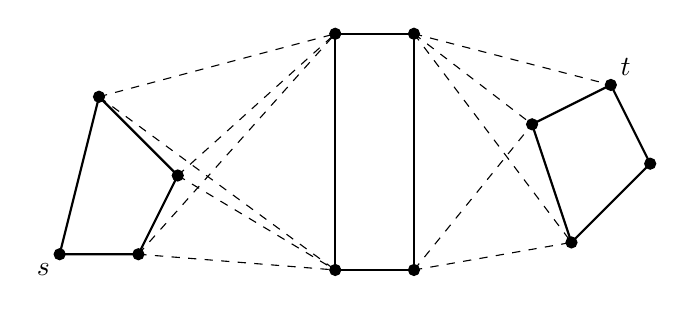
\begin{tikzpicture}
    % Variablen für das erste Polygon
    \coordinate (a0) at (0.5,0+0.2);
    \coordinate (a1) at (1,2+0.2);
    \coordinate (a2) at (2,1+0.2);
    \coordinate (a3) at (1.5,0+0.2);

    \filldraw (a0) circle (2pt);
    \filldraw (a1) circle (2pt);
    \filldraw (a2) circle (2pt);
    \filldraw (a3) circle (2pt);

    % Zeichne das erste Polygon
    \draw[thick] (a0) -- (a1) -- (a2) -- (a3) -- cycle;
    \node at (a0) [below left] {$s$};

    % Variablen für das Rechteck in der Mitte
    \coordinate (b0) at (4,0);
    \coordinate (b1) at (4,3);
    \coordinate (b2) at (5,3);
    \coordinate (b3) at (5,0);

    \filldraw (b0) circle (2pt);
    \filldraw (b1) circle (2pt);
    \filldraw (b2) circle (2pt);
    \filldraw (b3) circle (2pt);

    % Zeichne das Rechteck in der Mitte
    \draw[thick] (b0) -- (b1) -- (b2) -- (b3) -- cycle;


    % Variablen für das letzte Polygon
    \coordinate (c0) at (7,0+0.35);
    \coordinate (c1) at (8,1+0.35);
    \coordinate (c2) at (7.5,2+0.35);
    \coordinate (c3) at (6.5,1.5+0.35);

    \filldraw (c0) circle (2pt);
    \filldraw (c1) circle (2pt);
    \filldraw (c2) circle (2pt);
    \filldraw (c3) circle (2pt);

    % Zeichne das letzte Polygon
    \draw[thick] (c0) -- (c1) -- (c2) -- (c3) -- cycle;

    \node at (c2) [above right] {$t$};

    \draw[dashed] (a1) -- (b0);
    \draw[dashed] (a1) -- (b1);

    \draw[dashed] (a2) -- (b0);
    \draw[dashed] (a2) -- (b1);

    \draw[dashed] (a3) -- (b0);
    \draw[dashed] (a3) -- (b1);

    \draw[dashed] (b2) -- (c0);
    \draw[dashed] (b2) -- (c2);
    \draw[dashed] (b2) -- (c3);

    \draw[dashed] (b3) -- (c0);
    \draw[dashed] (b3) -- (c3);
  \end{tikzpicture}
  \caption{Beispiel Euclidean Shortest Path Problem}
  \label{fig:graphs:eulcidian_shotest_path_problem}
\end{figure}

\subsection{Eigenschaften}

Sichtbarkeitsgraphen sind im Allgemeinen \emph{nicht planar}.
Sie sind \emph{ungerichtet}, da die Sichtbarkeit zwischen zwei Punkten in beide Richtungen gilt.
Da die Gewichte der Kanten dem euklidischen Abstand zwischen den verbundenen Punkten entsprechen, bildet dieser eine untere Schranke des Abstandes für alle Knotenpaare, da ein kürzester Pfad durch das Umgehen von Hindernissen nur länger werden kann.

\subsection{Abgrenzung zu Straßengraphen}\label{graphs:strassengraphen}

Straßengraphen stellen eine spezielle Klasse von Graphen dar.
Eines ihrer auffälligsten Merkmale ist, dass sie nahezu planar sind, wobei Ausnahmen in Form von Brücken und Tunneln existieren.
Die Kantengewichte können etwa dem Luftlinienabstand oder der Reisezeit entsprechen, wobei sich letztere im Verlauf der Zeit ändert, etwa durch Stau oder Bauarbeiten.
Sie haben einen relativ geringen durchschnittlichen Knotengrad, denn Kreuzungen von mehr als zwei Straßen sind selten.

Sie besitzen eine hierarchische Struktur: Einfach gesagt, je schneller auf einer Straße gefahren werden darf, desto wichtiger ist diese für das Finden von kürzesten Pfaden.
Die Wichtigkeit der benutzten Straßen eines kürzesten Pfades steigt im Allgemeinen an, bis etwa eine Autobahn erreicht wird, und nimmt schließlich wieder ab, bis das Ziel erreicht wird.

Eine weitere Eigenschaft dieser hierarchischen Struktur ist, dass hinreichend lange Pfade durch ein vergleichsweise kleines Hitting-Set abgedeckt werden können, etwa durch alle Autobahnkreuze und Anschlussstellen.
Diese Beobachtung führt zur Definition der \emph{Highway Dimension}, einem Konzept, das von \cite{abraham2010highway} eingeführt wurde.

Aufgrund der unterschiedlichen Strukturen von Sichtbarkeitsgraphen und Straßengraphen können Algorithmen, die für Straßengraphen gute Laufzeiten aufweisen, zwar auf Sichtbarkeitsgraphen angewendet werden, allerdings ist ihre Rechenzeit häufig zu hoch, um eine effiziente Verarbeitung zu ermöglichen.

\subsection{Triangulierung}

Um die Distanzen zwischen Knotenpaaren in Sichtbarkeitsgraphen mit einer oberen Schranke abzuschätzen, kann eine \emph{Triangulierung} des Graphs durchgeführt werden, wie beispielsweise durch eine Delaunay-Triangulierung.
Dieser Ansatz kann jedoch lange, schmale Dreiecke erzeugen, die anschließend beseitigt werden können, um eine bessere obere Schranke zu erhalten.
Das Verfahren zur Erstellung der in dieser Arbeit verwendeten Triangulierung wurde ausführlich von Funke et al. \cite{funkescalable} beschrieben.

Die Knoten eines triangulierten Graphen $G_g$ bilden hierbei eine Obermenge zur Menge der Knoten des dazugehörigen Sichtbarkeitsgraphen $G_v$.
Die Triangulation darf den kürzesten Pfad Abstand zweier Knoten $a, b$ nicht verkleinern, aber vergrößern.
\autoref{fig:thessaloniki_comparison} vergleicht einen Sichtbarkeitsgraphen und dessen Triangulierung anhand eines Ausschnitts.

\begin{figure}[h!]%
  \centering
  \subfloat[\centering aegaeis-graph]{{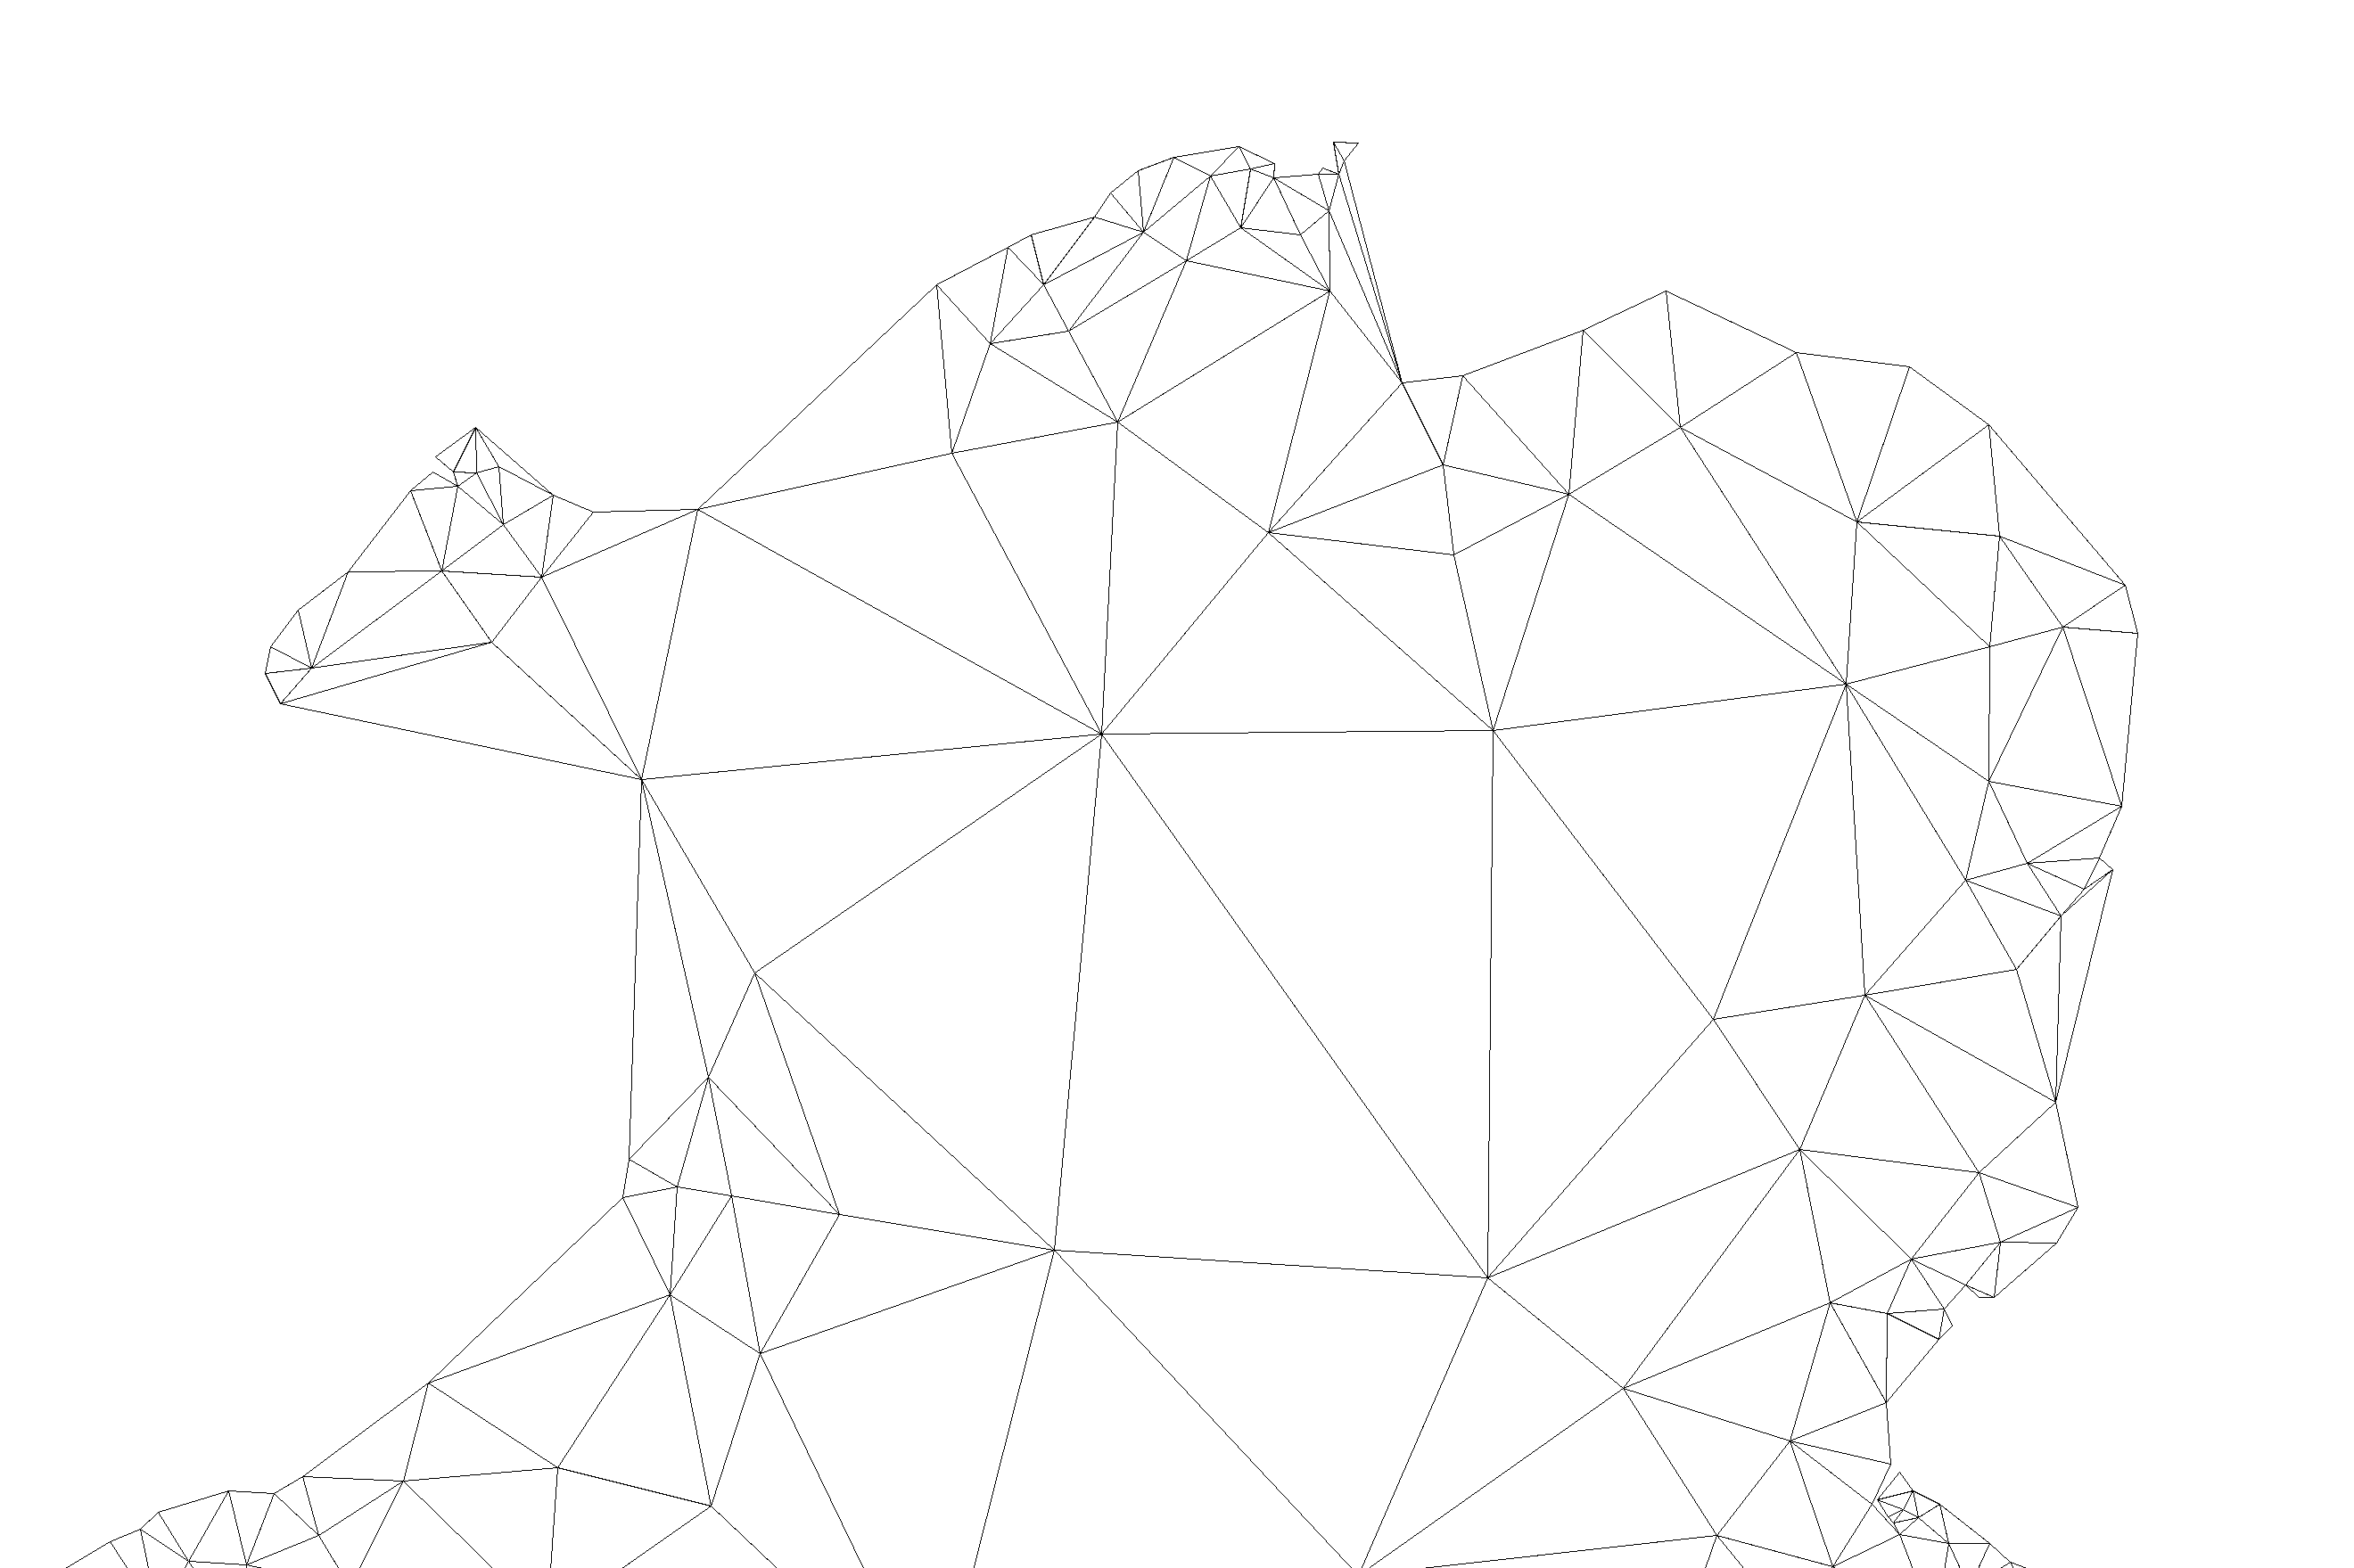
\includegraphics[width=.5\linewidth - 0.25cm]{img/thessaloniki-graph.png} }}%
  %\qquad
  \subfloat[\centering aegaeis-visibility]{{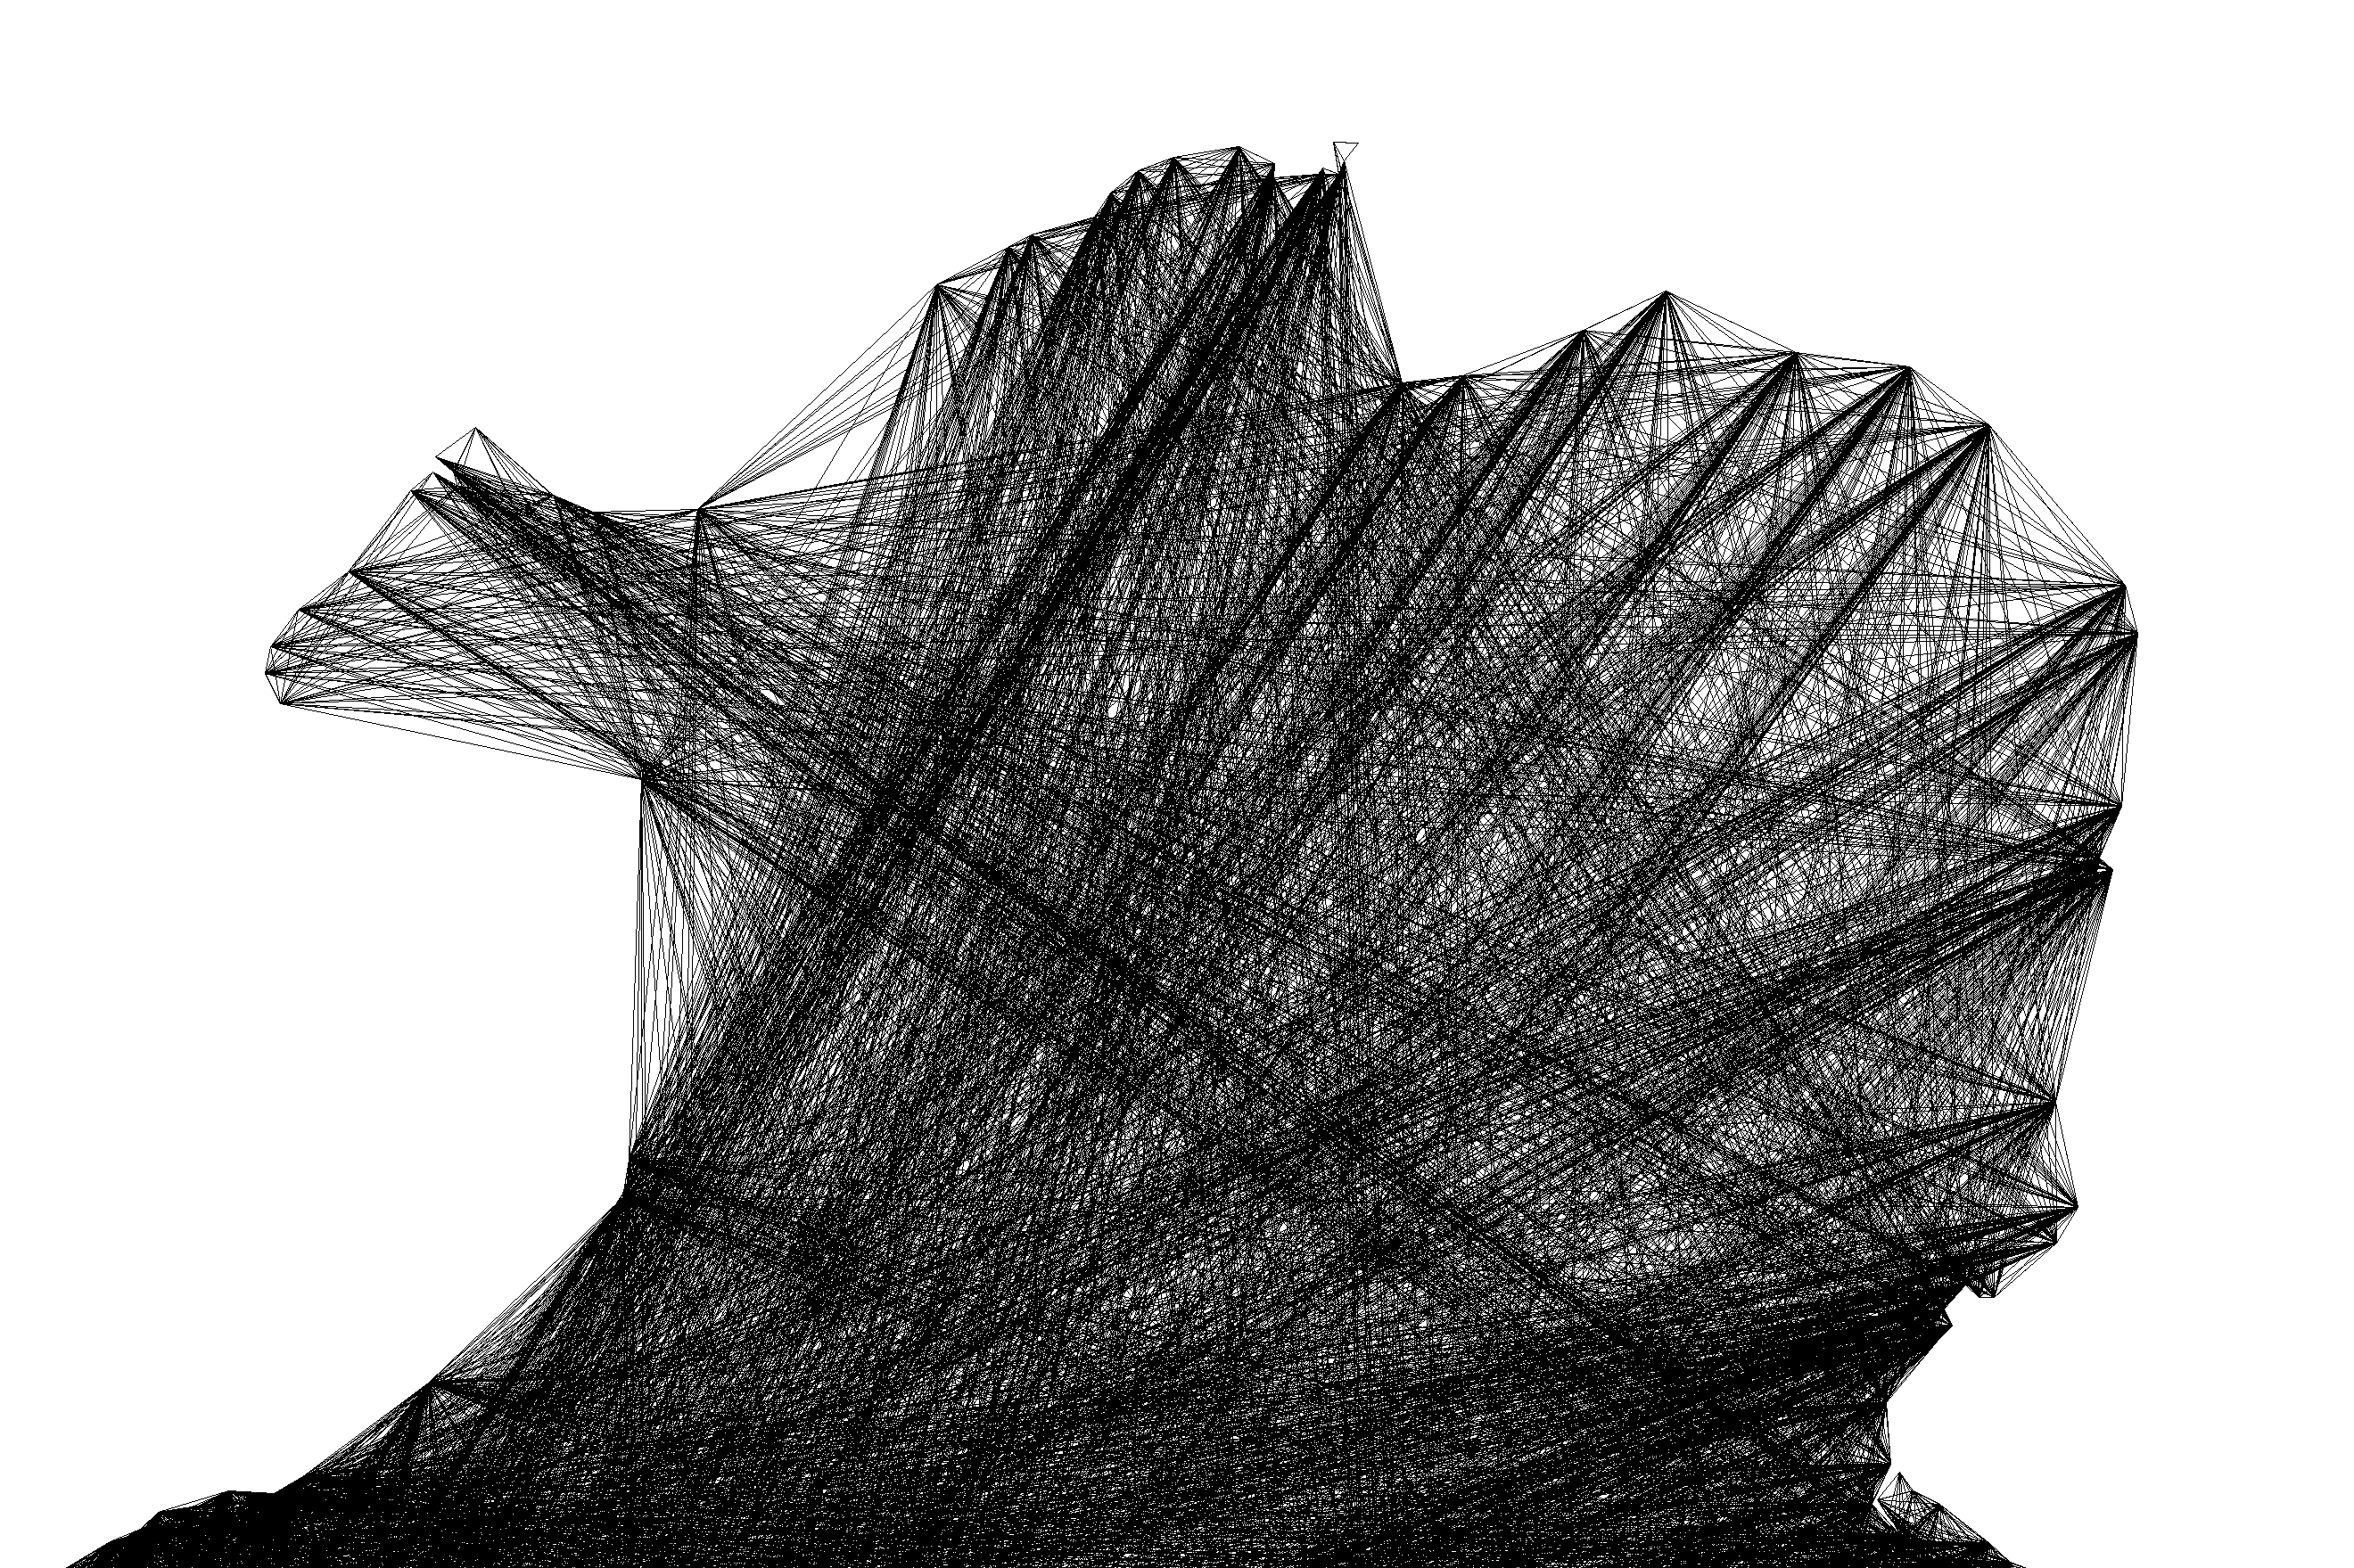
\includegraphics[width=.5\linewidth - 0.25cm]{img/thessaloniki-visibility.png} }}%
  \caption{Hafen von Thessaloniki}%
  \label{fig:thessaloniki_comparison}%
\end{figure}
